\section{Organización de los resultados}
Como se explicó en los capítulos anteriores, las propuestas planteadas consisten en modificar el paisaje de búsqueda del problema y utilizar 
una metaheurística simple, la búsqueda local iterada (ILS), para tratar de encontrar soluciones de alta calidad en tiempos reducidos.
%
Se plantean modificaciones en relación a la representación de las soluciones, la estructura de vecindad y la función de fitness.

En primer lugar se presentan resultados utilizando componentes estándar. 
%
En concreto, se usa la representación basada en permutaciones con vecindad N7, y el makespan como función de fitness.
%
A continuación se incluyen secciones para analizar el efecto de la función de fitness, la extensión planteada a la vecindad N7 y por último 
la representación basada en llaves aleatorias junto con la nueva vecindad propuesta. 
%
Se asignan acrónimos a cada variante para facilitar la comparación:

\begin{enumerate}
    \item \textbf{PN7Cmax} Representación basada en permutaciones, vecindad N7 y makespan como función de fitness.
    \item \textbf{PN7*} Representación basada en permutaciones, vecindad N7 y diversas funciones de fitness.
    \item \textbf{PN7extTup} Representación basada en permutaciones, vecindad N7 extendida y tupla ordenada de tiempos de finalización como función de fitness.
    \item \textbf{RpKeTup} Representación basada en llaves aleatorias, vecindad propuesta y tupla ordenada de tiempos de finalización como función de fitness.
\end{enumerate}

Cada una de las variaciones propuestas se ejecutó durante 5 minutos por 50 veces para cada instancia del conjunto \textbf{DMU01-80} con el fin de obtener 
un conjunto de resultados para comparar.

Puesto que el objetivo de las modificaciones planteadas en este trabajo es presentar una alternativa simple a los métodos del estado del arte pero 
sin perder demasiada calidad en las soluciones, se presenta la mediana del error relativo respecto al mejor resultado reportado en la literatura. 
%
El mejor resultado reportado en la literatura para cada instancia se muestra en el apéndice \ref{tab:sota}.
%
El error relativo se calcula entonces de la siguiente 
manera: \[\text{error relativo}= \frac{\text{makespan de la solución encontrada}-\text{mejor makespan en la literatura}}{\text{\text{mejor makespan en la literatura}}}\]

\section{Resultados para PN7Cmax}
Estos resultados sirven como una base para determinar si las modificaciones posteriores resultan en mejoras apreciables.
%
Se muestran los resultados de manera gráfica para facilitar su visualización. 
%
Los resultados detallados se encuentran en el apéndice \ref{app:resn7ils}. 

En la figura \ref{fig:PN7Cmax} podemos observar que la mediana del error relativo para la segunda mitad de las instancias es considerablemente 
mayor que para la primera mitad, en la cual en varios casos incluso se llegó a igualar el mejor resultado conocido.  
\begin{figure}[hbtp]
    \begin{subfigure}{\textwidth}
        \centering
        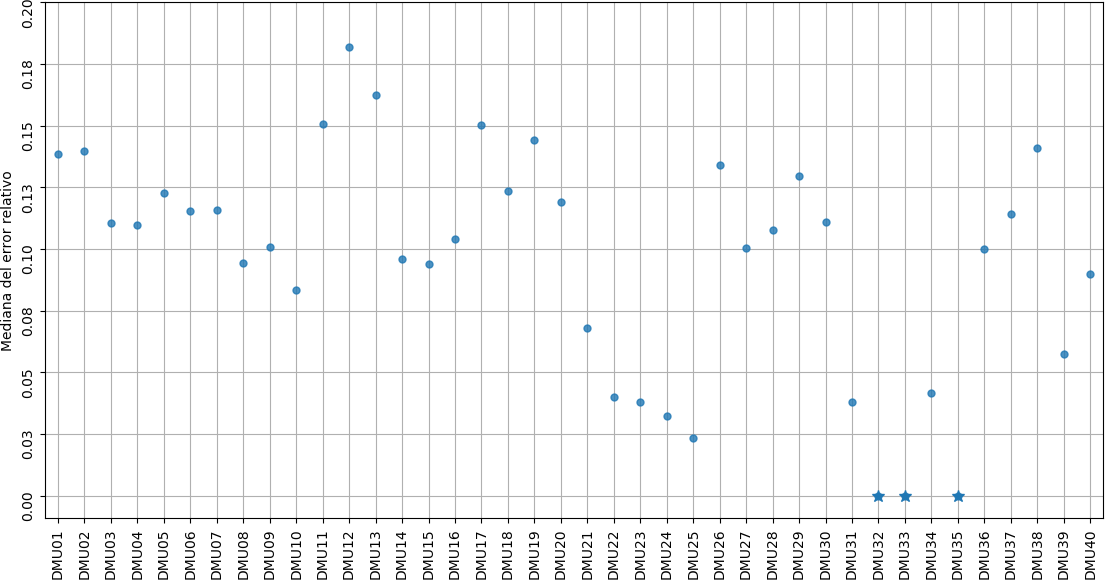
\includegraphics[scale=.65]{Imagenes/resn7ils1.png}
        \caption{Resultados para las instancias \textbf{DMU01-40}}
    \end{subfigure}
\end{figure}
\begin{figure}[H]\ContinuedFloat
    \begin{subfigure}{\textwidth}
        \centering
        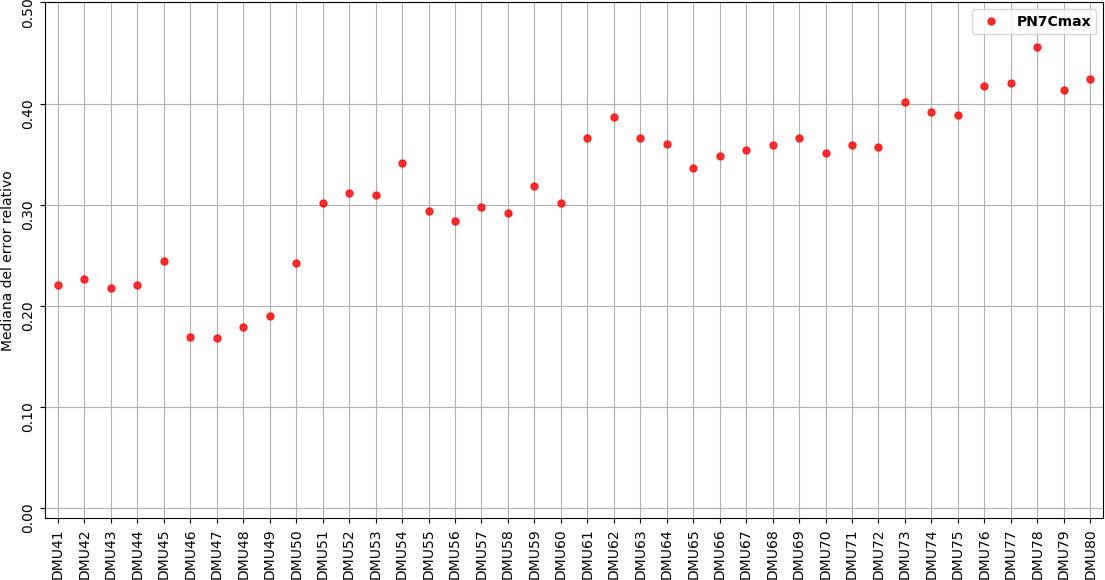
\includegraphics[scale=.65]{Imagenes/resn7ils2.png}
        \caption{Resultados para las instancias \textbf{DMU41-80}}
    \end{subfigure}
    \caption{Resultados para \textbf{PN7Cmax}. Se marcan los casos en los que se llegó a la mejor solución conocida.}
    \label{fig:PN7Cmax}
\end{figure}

Podemos observar que incluso usando una metaheurística simple por un corto tiempo podemos obtener resultados de calidad en gran cantidad de instancias. 
%
En la siguiente sección podremos observar que la función de fitness puede ayudarnos a tener incluso mejores resultados.

\section{Resultados para distintas funciones de fitness}
La función de fitness se obtiene al construir la dupla formada por el makespan y alguna característica adicional en ese orden. 
%
De esta forma, para comparar dos soluciones, se compara primero por makespan y en caso de empate por las siguientes características
de la dupla.

Con el objetivo de comparar los resultados de los diferentes métodos se considera exclusivamente el makespan alcanzado en cada instancia.
%
En particular, se comparan los resultados de cada instancia y si se encuentra que la diferencia entre dos métodos es estadísticamente significativa, 
se le suma un punto al método ganador (menor mediana) y se le resta uno al método perdedor. 
%
Sumando todos estos puntos, tenemos una puntuación global que permite realizar una ordenación de los métodos a comparar.
%
Para determinar si los conjuntos de resultados muestran diferencias estadísticamente significativas se utiliza la prueba de 
Wilcoxon con un nivel de significancia de $0.01$. 

\begin{table}[hbtp]
    \centering
\begin{tabular}{@{}cc@{}}
Característica                    & Acrónimo       \\ \hline \hline
$\mathbf{C_{max}}$ (makespan)     & \textbf{PN7Cmax}   \\\midrule
$\mathbf{\sum C_i^2}$             & \textbf{PN7C2}    \\\midrule
$\mathbf{\sum J_i}$               & \textbf{PN7Flow}  \\\midrule
$\mathbf{\sum I(C_i=C_{max})}$    & \textbf{PN7Icmax} \\\midrule
\textbf{Número de rutas críticas} & \textbf{PN7Rc}    \\\midrule
$\mathbf{Var(C_i)}$               & \textbf{PN7VarC}  \\\midrule
$\mathbf{(\{C_i\})}$              & \textbf{PN7Tup}    \\\midrule
\end{tabular}
    \caption{Acrónimos asignados a cada característica}
    \label{tab:caracter}
\end{table}

Los acrónimos asignados a cada una de las variantes que resultan de tomar las características propuestas se muestran en la tabla \ref{tab:caracter}.
%
Los resultados para las propuestas descritas en la sección \ref{prop:fitness} pueden verse de manera condensada en la figura \ref{fig:fcomp}. 
%
La casilla $(i,j)$ muestra el número de instancias en que la variante $i$ fue mejor menos el número veces que fue peor que la variante $j$.
%
Se incluye también un método que usa una tupla construida con las características que obtuvieron mejores resultados: \textbf{PN7C2/Flow/VarC}. 
%
En la tabla \ref{tab:fcomp} se presentan ordenadas las variantes por el puntaje obtenido. 
%
Podemos observar que las primeras tres entradas tienen puntuaciones similares, y presentan diferencias grandes con las demás.

Podemos observar en la figura \ref{fig:fcomp} y en la tabla \ref{tab:fcomp} que el makespan fue la peor función de fitness. 
%
Para la tupla construida combinando las mejores características se observan pocas mejoras por lo que podemos concluir que agregar más características no lleva necesariamente a mejores resultados. Los mejores resultados se obtienen al construir la tupla de tiempos ordenados de finalización de las máquinas por lo que de ahora en adelante la función de fitness queda fija de esta manera y en los resultados subsecuentes solo se considera este caso. Los resultados detallados para esta función de fitness se muestran en el apéndice \ref{app:resn7tuple}.
Con estos resultados podemos concluir que es ventajoso enfocarse en mejorar las máquinas que tardan más tiempo siendo las tres mejores variantes las que toman más en cuenta estas máquinas.

\begin{figure}[hbtp]
    \centering
    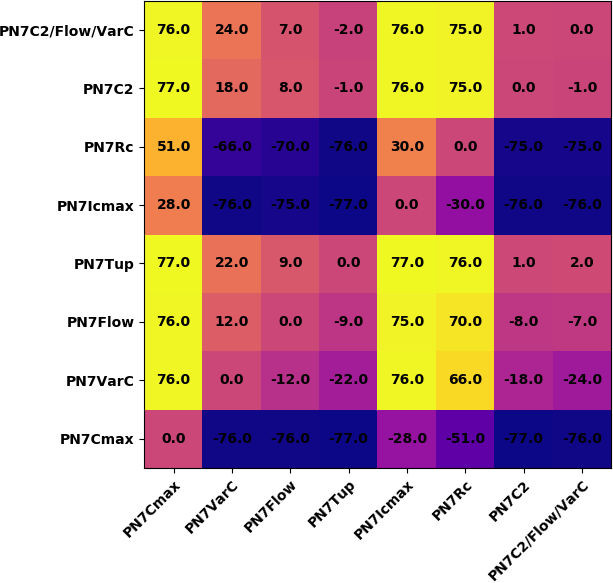
\includegraphics[scale=.8]{Imagenes/fitnesscomp.png}
    \captionof{figure}{Condensado de los resultados para las modificaciones a la función de fitness. }
    \label{fig:fcomp}
\end{figure}
\begin{table}[hbtp]
    \centering
\begin{tabular}{@{}cc@{}}
Variante & Puntaje \\ \midrule
\toprule
    \textbf{PN7Tup} & 264.0 \\ \midrule
    \textbf{PN7C2/Flow/VarC} & 257.0 \\ \midrule
    \textbf{PN7C2} & 252.0 \\ \midrule
    \textbf{PN7Flow} & 209.0 \\ \midrule
    \textbf{PN7VarC} & 142.0 \\ \midrule
    \textbf{PN7Rc} & -281.0 \\ \midrule
    \textbf{PN7Icmax} & -382.0 \\ \midrule
    \textbf{PN7Cmax} & -461.0 \\ \midrule
\end{tabular}
    \caption{Puntaje para cada una de las variantes de función de fitness propuesta}
    \label{tab:fcomp}
\end{table}

Para mostrar de manera más concisa el efecto de la función de fitness en la calidad de las soluciones encontradas, en la figura \ref{fig:PN7CmaxvsPN7Tup} se muestra una comparación de los resultados hallados para la mejor función de fitness \textbf{PN7Tup} contra el caso base \textbf{PN7Cmax} que fue el que obtuvo peores resultados.
%
Podemos ver que la mejora es estable, presentando menor mediana en todas las instancias salvo en las que ya se alcanzaban las mejores soluciones conocidas,
donde ambos métodos obtuvieron los mismos resultados.


\begin{figure}[hbtp]
    \begin{subfigure}{\textwidth}
        \centering
        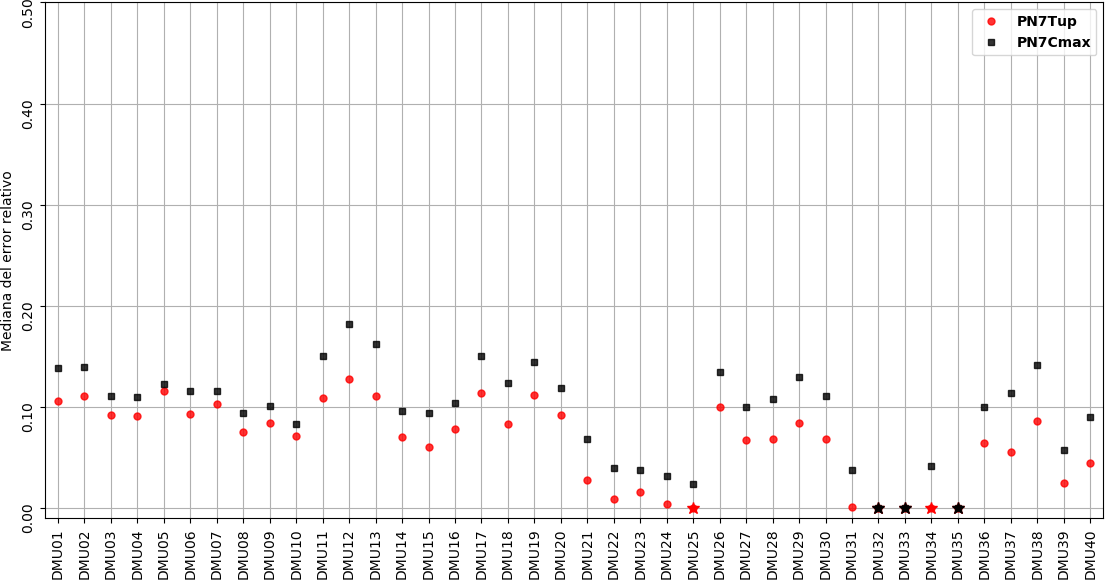
\includegraphics[scale=.65]{Imagenes/PN7CmaxvsPN7Tup_1.png}
        \caption{Resultados para las instancias \textbf{DMU01-40}}
    \end{subfigure}
\end{figure}
\begin{figure}[H]\ContinuedFloat
    \begin{subfigure}{\textwidth}
        \centering
        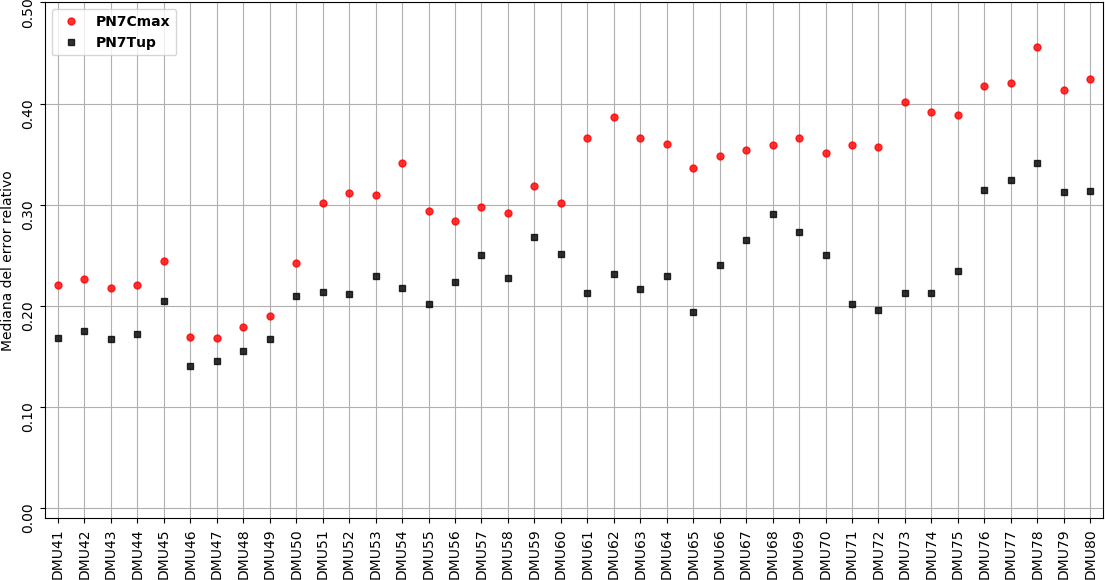
\includegraphics[scale=.65]{Imagenes/PN7CmaxvsPN7Tup_2.png}
        \caption{Resultados para las instancias \textbf{DMU41-80}}
    \end{subfigure}
    \caption{Comparación entre la peor y la mejor función de fitness. Se marcan los casos en los que se llegó a la mejor solución conocida.}
    \label{fig:PN7CmaxvsPN7Tup}
\end{figure}


\section{Resultados para PN7extTup}
Los resultados para la extensión de la vecindad N7 que considera movimientos que buscan aprovechar espacios de inactividad de las máquinas, se 
comparan con los mejores mostrados en la sección pasada (\textbf{PN7Tup}).
%
Se sigue el mismo procedimiento que en la sección anterior para hacer esta comparación.
%
En la figura \ref{fig:n8vsn7} podemos observar que \textbf{PN7extTup} tiene una puntuación total de 28 (cantidad de instancias en que gana menos cantidad
de instancias en que pierde), por lo que la tendencia general es positiva.
%
Sin embargo, en la figura \ref{fig:errn8vsn7} podemos observar que la mejora no es robusta ya que en algunos casos resulta significativamente 
peor que \textbf{PN7Tup}. 
%
Por ello, esta extensión se debe considerar como una alternativa de vecindad, y no como una mejora.
%
Los resultados detallados para la \textbf{PN7extTup} se encuentran en el apéndice \ref{app:resn8tuple}.


\begin{figure}[hbtp]
    \centering
    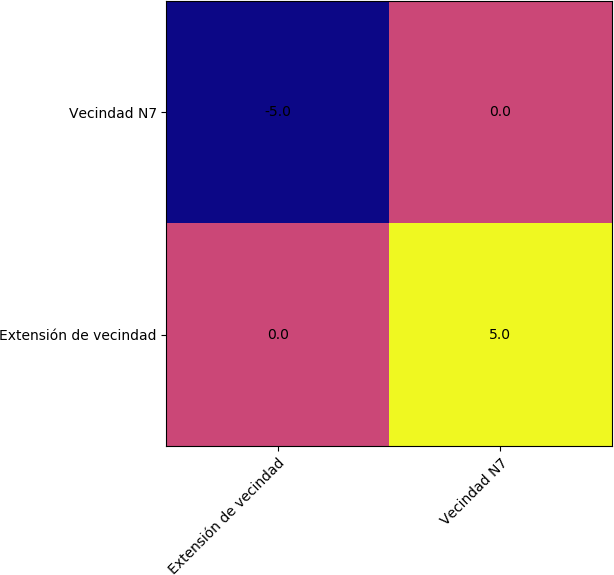
\includegraphics[scale=.7]{Imagenes/n8vsn7.png}
    \caption{Resultados de la comparación}
    \label{fig:n8vsn7}
\end{figure}

\begin{figure}[hbtp]
    \begin{subfigure}{\textwidth}
        \centering
        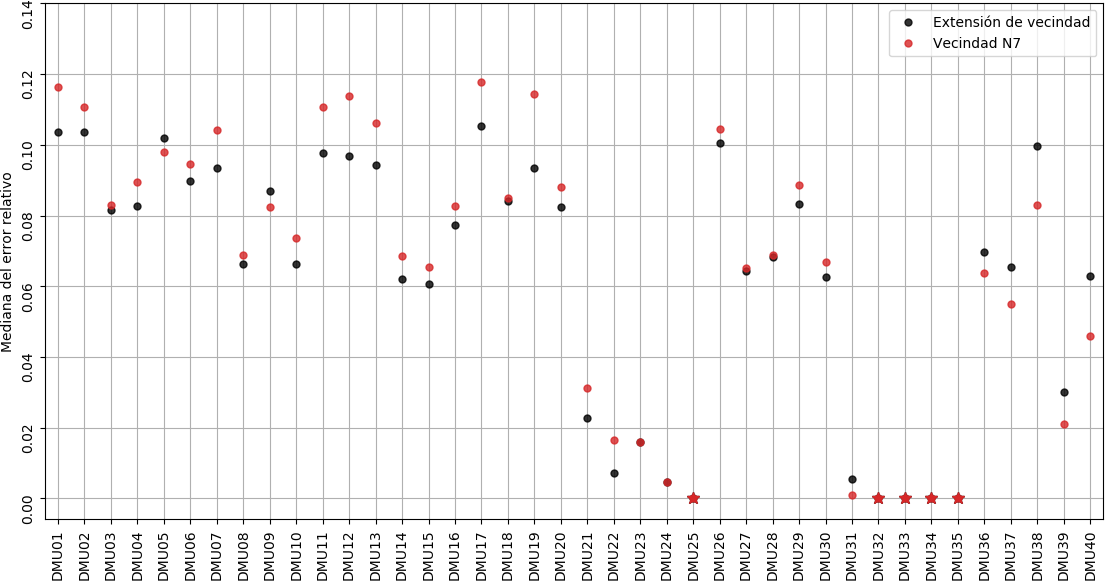
\includegraphics[scale=.6]{Imagenes/n8vsn7err1.png}
        \caption{Resultados para las instancias \textbf{DMU01-40}}
    \end{subfigure}
\end{figure}
\begin{figure}[H]\ContinuedFloat
    \begin{subfigure}{\textwidth}
        \centering
        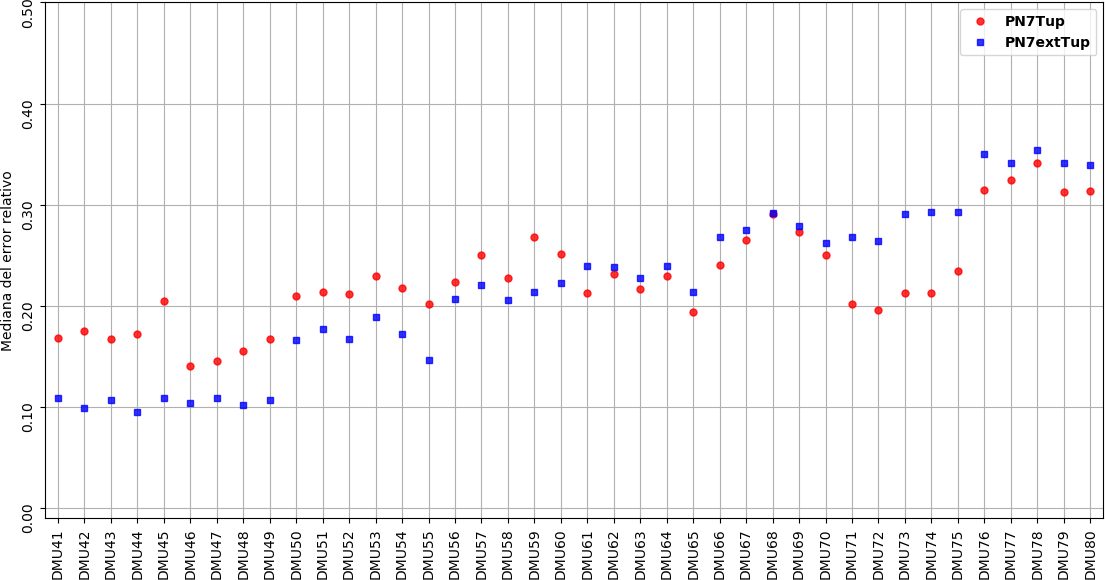
\includegraphics[scale=.6]{Imagenes/n8vsn7err2.png}
        \caption{Resultados para las instancias \textbf{DMU41-80}}
    \end{subfigure}
    \caption{Resultados para los métodos \textbf{PN7extTup} y \textbf{PN7Tup}. Se marcan los casos en los que se llegó a la mejor solución conocida.}
    \label{fig:errn8vsn7}
\end{figure}

\section{Cambio de representación y vecindad}
El cambio de representación y vecindad \textbf{RpKeTup} se compara con las dos propuestas previas: \textbf{PN7extTup} y \textbf{PN7Tup}. Se sigue el mismo procedimiento mencionado anteriormente para comparar y determinar si existe una diferencia significativa entre los resultados obtenidos. En la figura \ref{fig:n7vsn8vspr} y en la tabla \ref{tab:n7n8pr} podemos apreciar que \textbf{RpKeTup} presenta una ventaja aunque no muy grande. Los resultados detallados para \textbf{RpKeTup} se encuentran en el apéndice \ref{app:resprtuple}. 

\begin{figure}[hbtp]
    \centering
    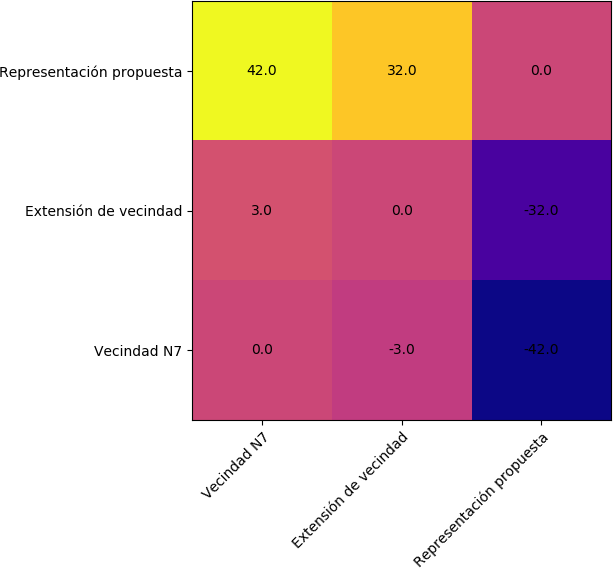
\includegraphics[scale=.7]{Imagenes/prn7n8comp.png}
    \caption{Resultados de la comparación entre los tres métodos.}
    \label{fig:n7vsn8vspr}
\end{figure}

\begin{table}[hbtp]
    \centering
\begin{tabular}{@{}cc@{}}
Variante & Puntaje \\ \midrule
\toprule
    \textbf{RpKeTup} & 37.0 \\ \midrule
    \textbf{PN7extTup} & 30.0 \\ \midrule
    \textbf{PN7Tup} & -67.0 \\ \midrule
\end{tabular}
    \caption{Puntaje total para cada método.}
    \label{tab:n7n8pr}
\end{table}

En la figura \ref{fig:n7vsn8vsprerr} podemos observar que la ventaja que tiene \textbf{RpKeTup} está concentrada en la segunda mitad de las instancias. 
%
Como se mencionó anteriormente, en las instancias \textbf{DMU41-80} todos los trabajos tienen operaciones iniciales en un mismo subconjunto de máquinas; 
%
la nueva representación toma en cuenta soluciones activas con lo que consigue evitar parcialmente el cuello de botella que resulta en soluciones de muy mala calidad,
reduciendo significativamente el error relativo.
%
Se puede concluir entonces que al menos para las instancias más difíciles, la nueva propuesta consigue mejoras muy significativas.
\begin{figure}[hbtp]
    \begin{subfigure}{\textwidth}
        \centering
        %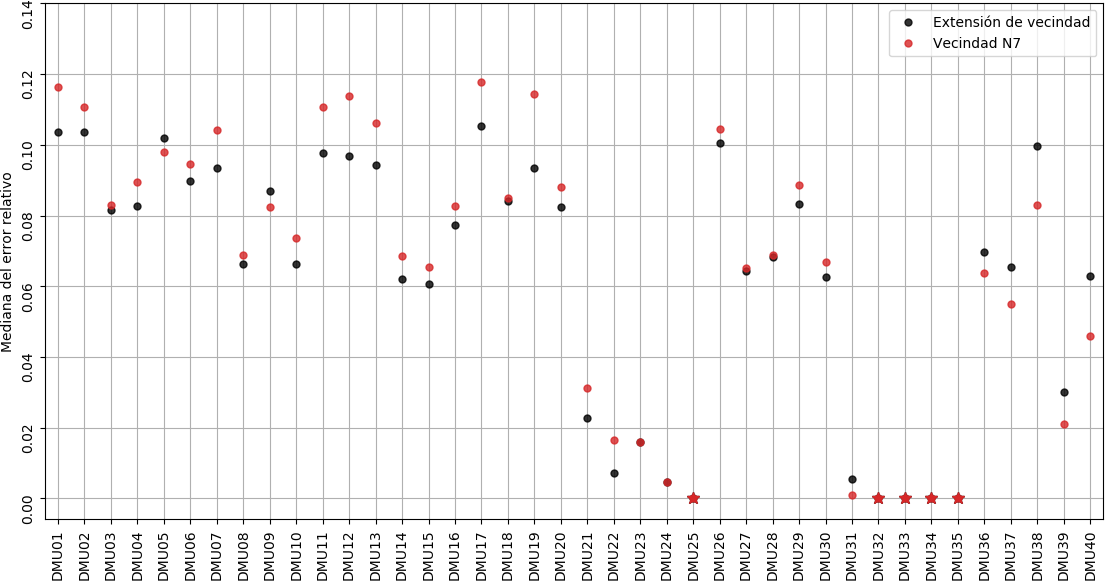
\includegraphics[height=.78\textwidth,width=.95\textheight,angle=270]{Imagenes/n8vsn7err1.png}
        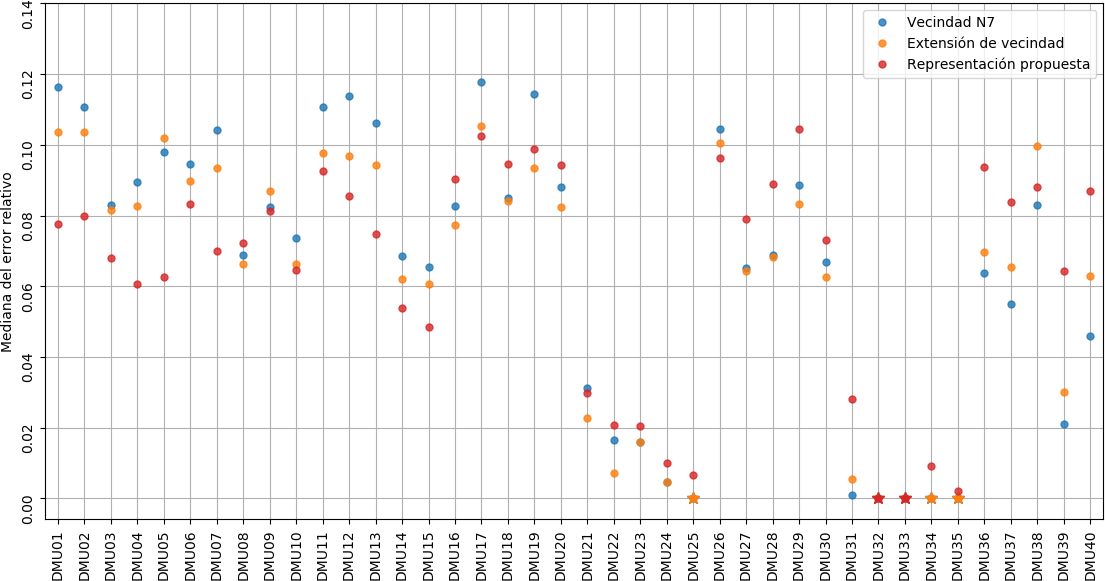
\includegraphics[scale=.6]{Imagenes/prvsn7vsn8err1.png}
        \caption{Resultados para las instancias \textbf{DMU01-40}}
    \end{subfigure}
\end{figure}
\begin{figure}[H]\ContinuedFloat
    \begin{subfigure}{\textwidth}
        \centering
        %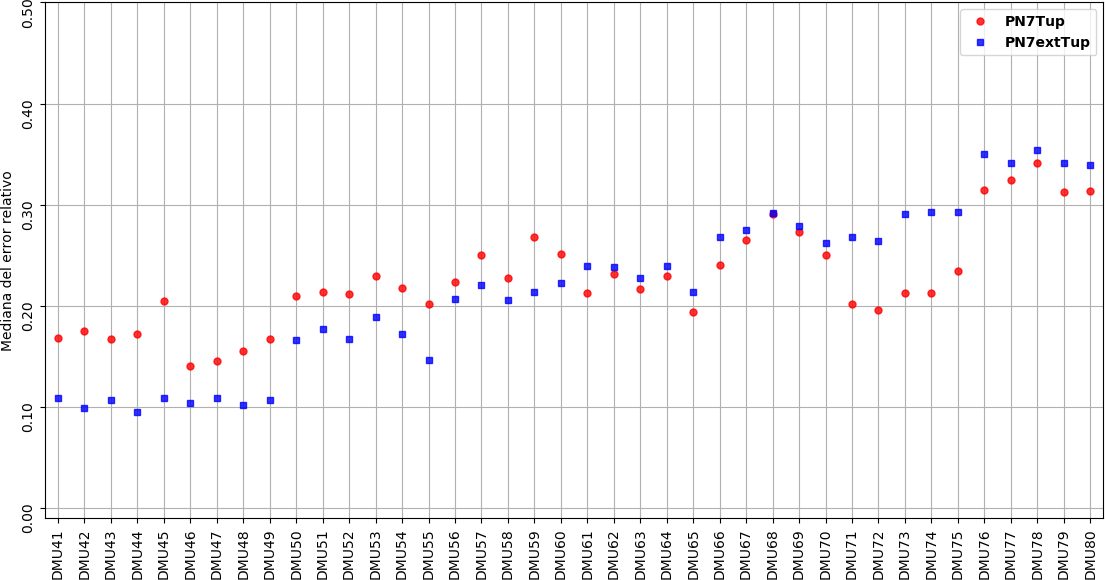
\includegraphics[height=.78\textwidth,width=.95\textheight,angle=270]{Imagenes/n8vsn7err2.png}
        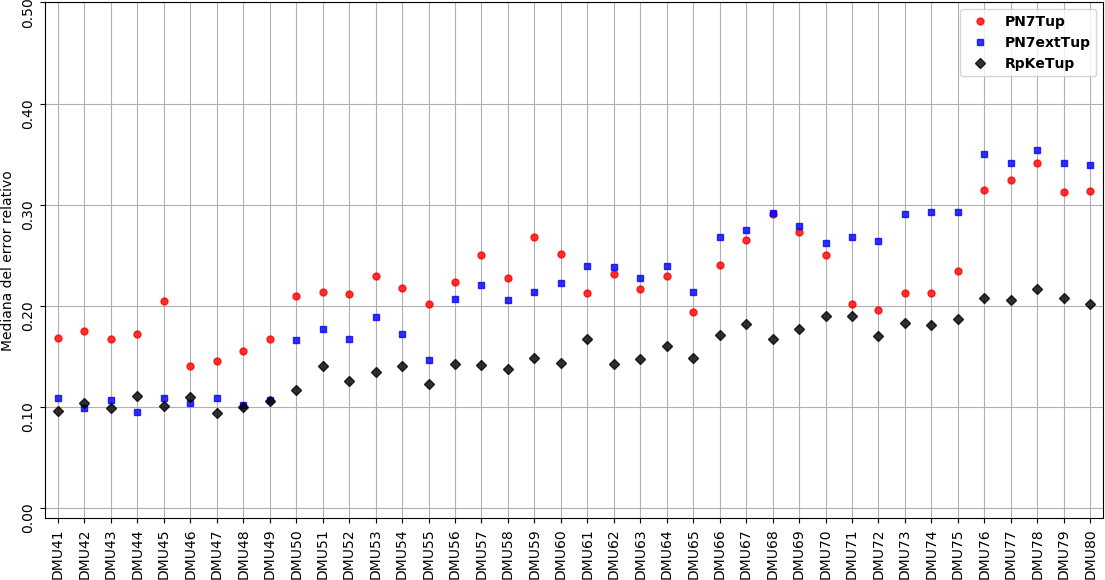
\includegraphics[scale=.6]{Imagenes/prvsn7vsn8err2.png}
        \caption{Resultados para las instancias \textbf{DMU41-80}}
    \end{subfigure}
    \caption{Resultados para \textbf{PN7Tup}, \textbf{PN7extTup} y \textbf{RpKeTup}. Se marcan los casos en los que se llegó a la mejor solución conocida.}
    \label{fig:n7vsn8vsprerr}
\end{figure}

Para resaltar las diferencias entre \textbf{RpKeTup} y \textbf{PN7Tup} se tomó la instancia en la que se obtuvieron los resultados más dispares 
(\textbf{DMU78}) y para cada óptimo local visitado se registró su makespan así como el tamaño de su vecindad como se muestra en la figura \ref{fig:mattgraph}. 
%
Este procedimiento nos permite hacernos una idea de cómo se conectan las soluciones en función de su makespan. 
%
Lo más deseable es que los óptimos locales de alta calidad tengan vecindades grandes y los de mala calidad tengan vecindades pequeñas, 
de modo que sea fácil llegar a una solución de buena calidad y difícil obtener una de mala calidad. 
%
En la figura \ref{fig:mattgraph} podemos ver se tiene una tendencia opuesta a la deseada, es decir, que el tamaño de la vecindad de una 
solución decrece junto con el makespan. i
%
En particular, no hay soluciones con makespan pequeño y más de 1000 vecinos; 
%
sin embargo, esa situación sí se da al considerar valores de makespan más grandes.
%
El patrón bandeado que se observa en la figura \ref{fig:mattgraph} para \textbf{PN7Tup} posiblemente se deba a la dependencia que tiene el 
tamaño de la vecindad de una solución con su número de rutas críticas ya que en \textbf{RpKeTup} esto no se observa.
%
Además, es notorio que \textbf{RpKeTup} tiene vecindades más grandes y su tamaño no depende en gran medida del makespan, lo que ayuda a obtener soluciones
de mayor calidad.

\begin{figure}[hbtp]
    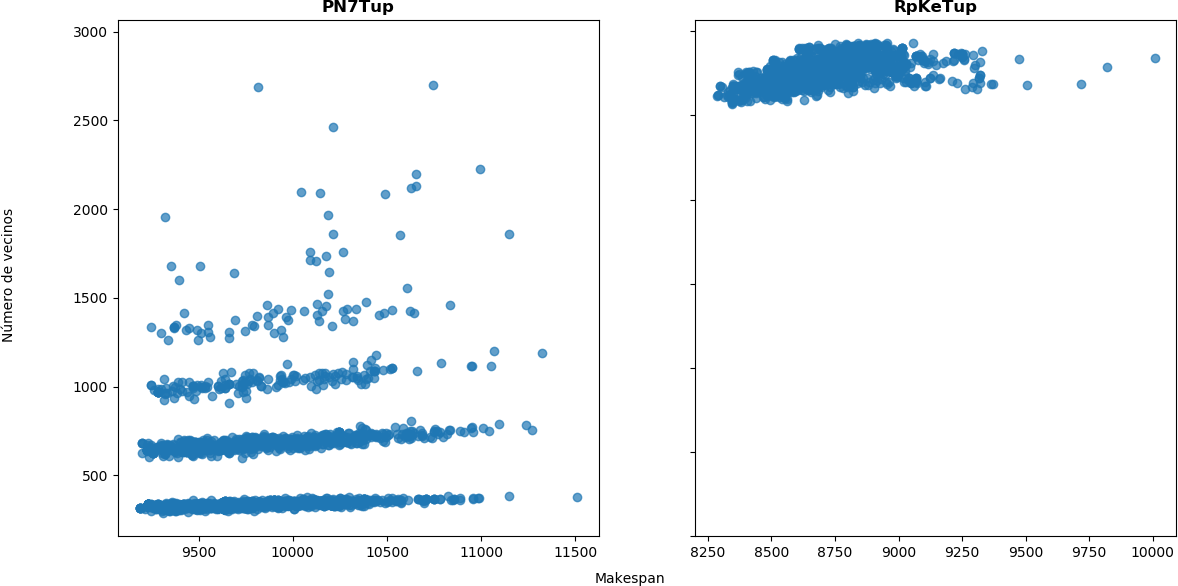
\includegraphics[scale=.6]{Imagenes/compvec78.png}
    \caption{Comparación de tamaño de la vecindad contra makespan de los óptimos locales para la instancia \textbf{DMU78} }
    \label{fig:mattgraph}
\end{figure}

Otro modo de visualizar las diferencias entre ambas representaciones es al fijarnos en los alrededores de un óptimo local. 
%
Entre más parecido sea el makespan de un óptimo local al de sus vecinos, más suave es el paisaje de búsqueda. Podemos visualizar esto mediante diagramas de caja de 
la diferencia relativa del makespan de los óptimos locales con sus vecinos. 

En las figuras \ref{fig:bxp1} y \ref{fig:bxp2} observamos que los vecinos de los óptimos locales para \textbf{RpKeTup} son más parecidos que los de \textbf{PN7Tup}, esto nos indica que el paisaje de búsqueda es más suave para \textbf{RpKeTup} lo cual, como se ha mencionado antes, es ventajoso para las metaheurísticas de trayectoria.  

Este efecto se debe a que la representación basada en permutaciones considera movimientos que pueden ser bastante disruptivos, pues puede por ejemplo 
atrasar toda una cadena de operaciones dejando huecos grandes en la planificación, mientras que en la nueva representación basada en llaves aleatorias el proceso de decodificación mediante el algoritmo de Giffler Thompson \ref{alg:GT} evita que se generen estos huecos evitando transformaciones tan bruscas.
\begin{figure}[hbtp]
    \begin{subfigure}{\textwidth}
        \centering
        %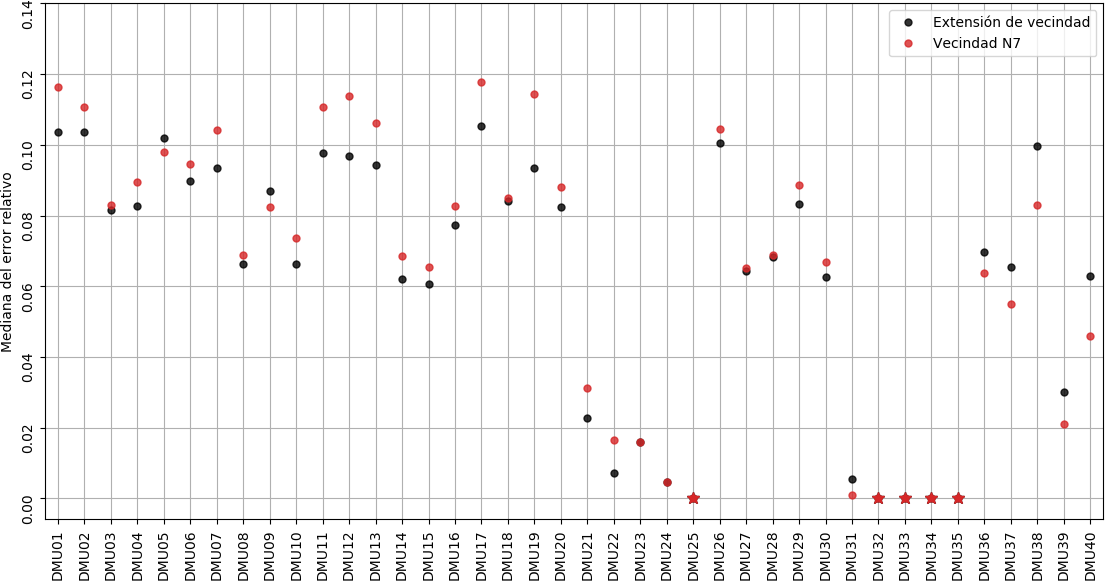
\includegraphics[height=.78\textwidth,width=.95\textheight,angle=270]{Imagenes/n8vsn7err1.png}
        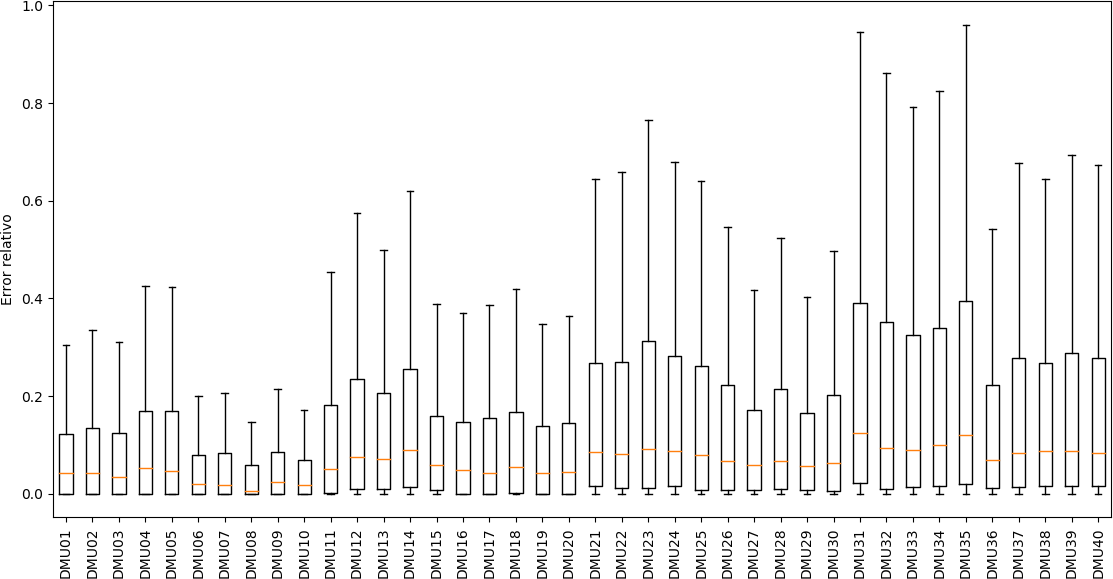
\includegraphics[scale=.6]{Imagenes/bxpn7_1.png}
        \caption{Representación original con vecindad n7 instancias \textbf{DMU01-40}}
    \end{subfigure}
\end{figure}
\begin{figure}[H]\ContinuedFloat
    \begin{subfigure}{\textwidth}
        \centering
        %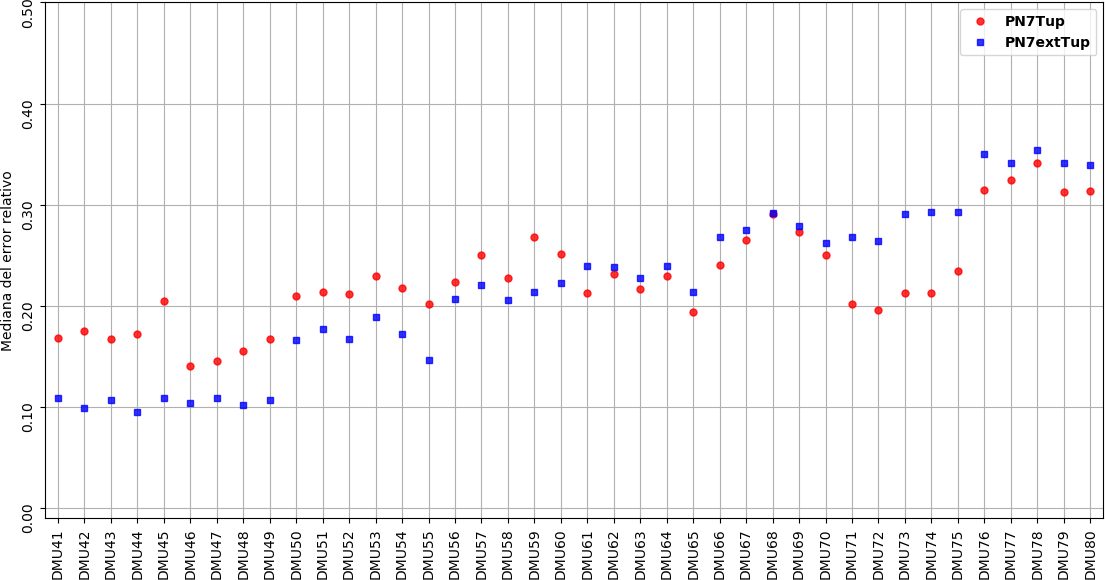
\includegraphics[height=.78\textwidth,width=.95\textheight,angle=270]{Imagenes/n8vsn7err2.png}
        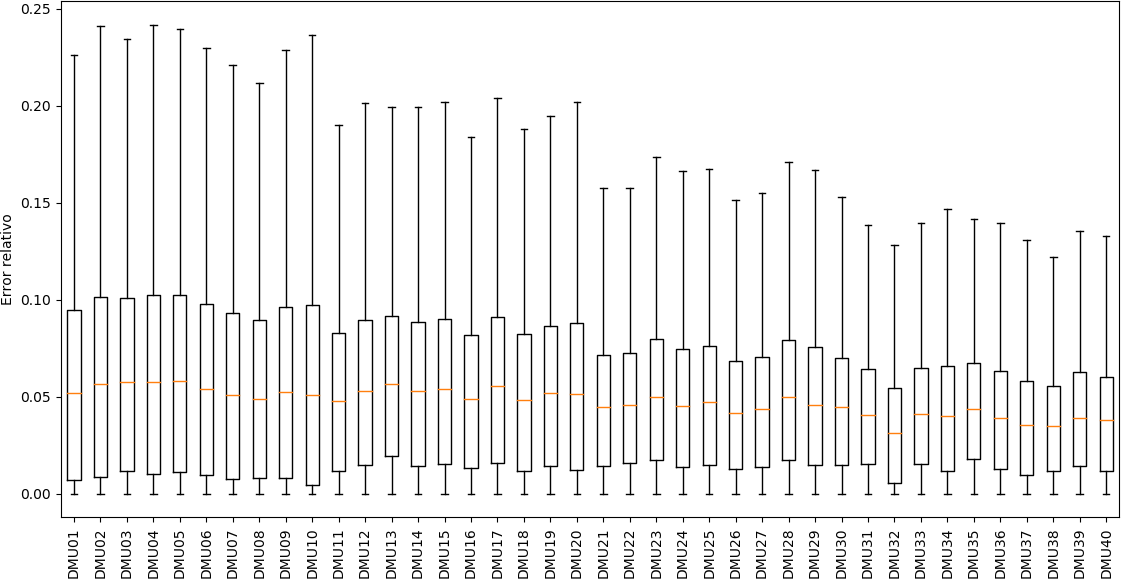
\includegraphics[scale=.6]{Imagenes/bxppr_1.png}
        \caption{Representación propuesta instancias \textbf{DMU01-40}}
    \end{subfigure}
    \caption{Diagramas de caja de la diferencia relativa en makespan de un óptimo local con sus vecinos}
    \label{fig:bxp1}
\end{figure}


\begin{figure}[hbtp]
    \begin{subfigure}{\textwidth}
        \centering
        %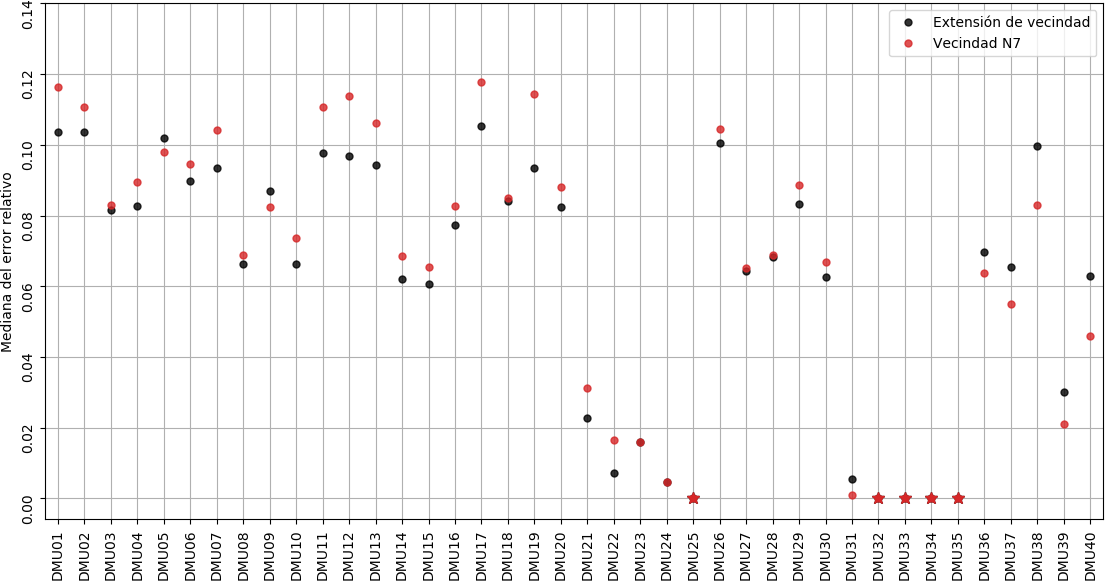
\includegraphics[height=.78\textwidth,width=.95\textheight,angle=270]{Imagenes/n8vsn7err1.png}
        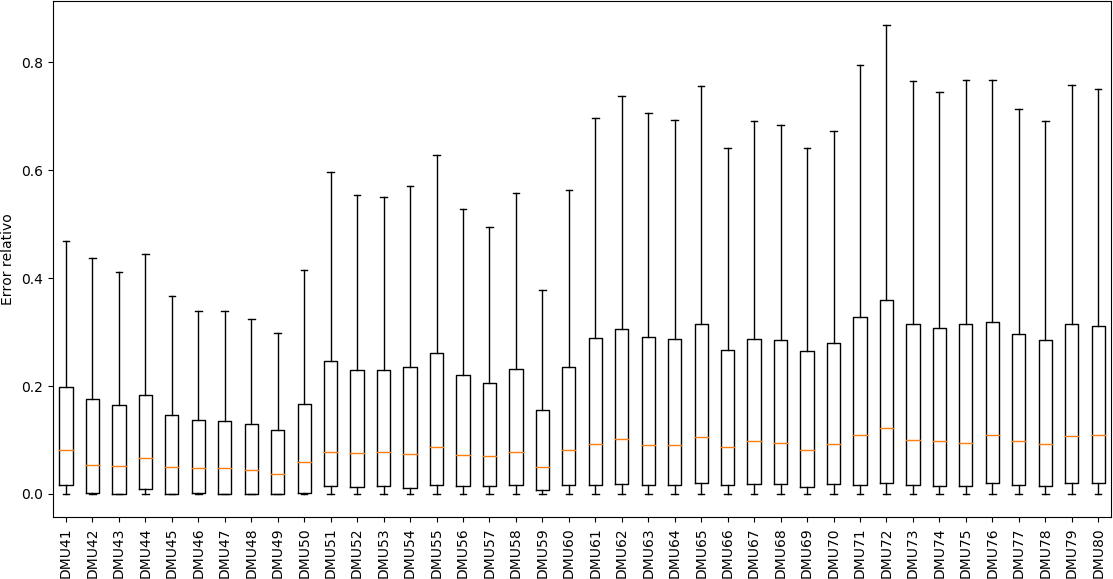
\includegraphics[scale=.6]{Imagenes/bxpn7_2.png}
        \caption{Representación original con vecindad n7 instancias \textbf{DMU41-80}}
    \end{subfigure}
\end{figure}
\begin{figure}[H]\ContinuedFloat
    \begin{subfigure}{\textwidth}
        \centering
        %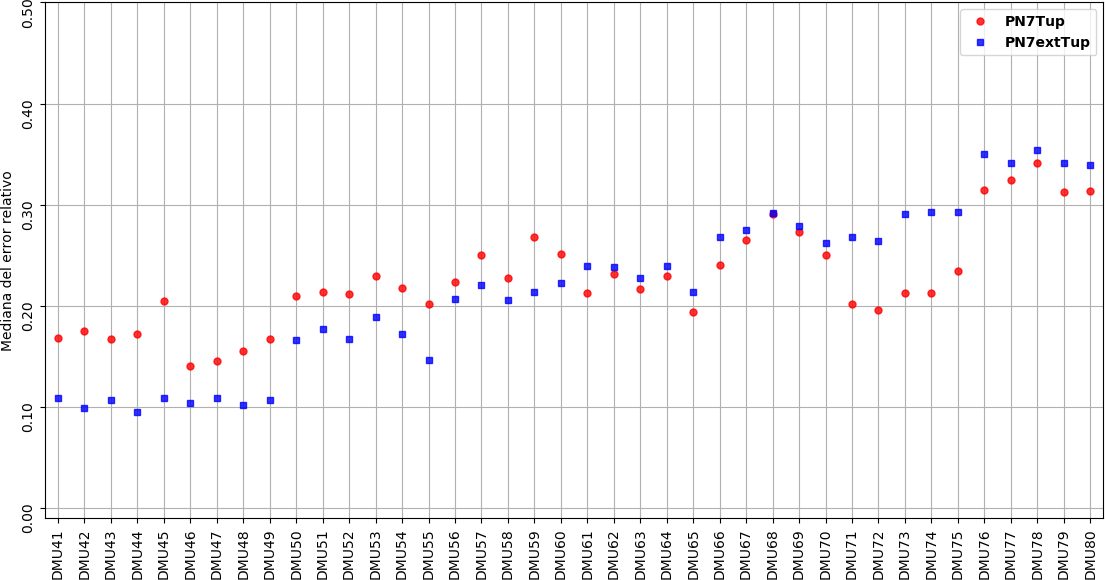
\includegraphics[height=.78\textwidth,width=.95\textheight,angle=270]{Imagenes/n8vsn7err2.png}
        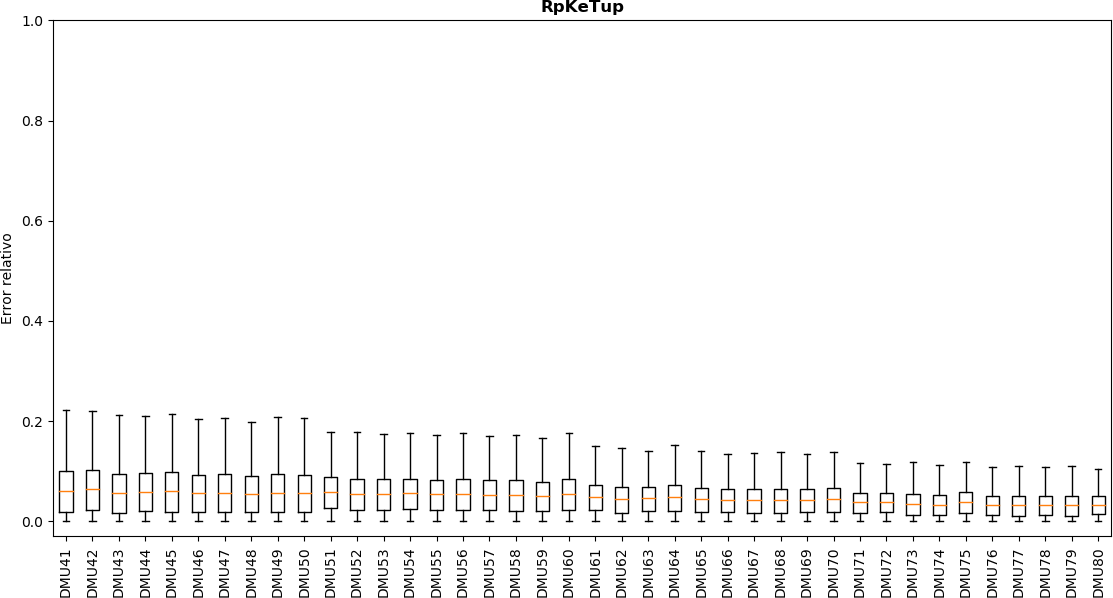
\includegraphics[scale=.6]{Imagenes/bxppr_2.png}
        \caption{Representación propuesta instancias \textbf{DMU41-80}}
    \end{subfigure}
    \caption{Diagramas de caja de la diferencia relativa en makespan de un óptimo local con sus vecinos}
    \label{fig:bxp2}
\end{figure}

